\chapter{Design, Segurança e Métricas de Software}
\label{cap-metrics}

\section{Design de Software}
\label{sec-design-sw}

O desenvolvimento de software é um processo complexo, pois envolve diversas etapas que visam o entendimento dos problemas a serem solucionados, o projeto de uma solução, a implementação desta solução, testes sobre o produto, dentre outros passos importantes e não menos complexos. As metodologias mais conhecidas de desenvolvimento de software tais como o Processo Unificado e o \emph{Extreme Programming} perpassam por essas etapas com diferentes focos e técnicas, ambos buscando a entrega de soluções em software que atendam aos problemas de seus clientes. Devida esta complexidade, tanto do processo quanto do produto de software, prazos e custos não devem ser os únicos fatores considerados para reger um projeto de software. Em complementação, a qualidade deve ser preponderante para o sucesso do produto que, além de resolver o problema, deve fazê-lo adequadamente segundo os atributos e critérios de qualidade estabelecidos para o projeto.

%

O \emph{design} se torna mais importante a medida que a complexidade dos softwares aumentam durante o desenvolvimento, pois suas consequências são diretas sobre os atributos de qualidade do software tais como flexibilidade, testabilidade, manutenibilidade, desempenho e segurança. Em projetos de software livre, por exemplo, estes atributos de qualidade são fatores fundamentais na atratividade de colaboradores para os projetos, onde se observa uma correlação entre métricas de qualidade de código-fonte com a atratividade desses projetos \cite{meirelles2013metrics}. 

%

Visando amenizar os riscos de se construir um sistema que não alcance seus objetivos, a arquitetura do software tem recebida atenção especial através dos métodos, práticas de desenvolvimento e estudos acadêmicos. O conjunto de decisões sobre as estruturas estáticas do sistema, hierarquia de módulos, descrição de dados, seleção de algoritmos, agrupamento e interface entre módulos podem ser previamente pensados a partir de modelos e documentação como também podem emergir a partir da aplicação de padrões de implementação e \emph{refactorings} sobre o código. O mais importante é que a medida que novas funcionalidades são incorporadas, o \emph{design} do código continue mantendo suas características, aplicando bons princípios e não sendo um impendimento para manutenção e evolução do software, comprometendo assim sua existência e utilização. Neste sentido, o Engenheiro de Software tem a responsabilidade de desenvolver o software sem degradar sua arquitetura, respeitando padrões estabelecidos, evoluindo seu \emph{design} à medida que implementa novas linhas de código e manter o código limpo e seguro para possibilitar que outros Engenheiros também compreendam e evoluam o software.

%

Nesta seção apresentaremos os princípios reconhecidos de bom \emph{design} e algumas formas como estes princípios podem ser aplicados no código-fonte. Posteriormente, identificamos como as decisões de design são observáveis em termos de \emph{Bad Smells} e Código Limpo. Neste sentido, pretendemos estudar e revisar como estas características observáveis possuem relação com métricas de monitoramento de código-fonte com objetivo de prover mecanismos que permitam ao Engenheiro de Software e gestores destinarem seus esforços na remoção de não-conformidades e evolução do software.

%

\subsection{O Design, Princípios e Práticas}
\label{sec-principles-practises}

O \emph{design} do software consiste no conjunto de decisões importantes tomadas sobre a organização de um sistema de software que podem ser observadas e mapeadas em diferentes níveis de abstração no código-fonte e em outros produtos. Katki (\citeyear{katki1991}) completa a definição explicando que \emph{design} é tanto o processo de definição da arquitetura, módulos, interfaces e outras características de um sistema quanto o resultado deste processo. Para comunicação e documentação pode-se ter modelos que representem o \emph{design} conceitual demonstrando, por exemplo, o estilo arquitetural adotado na aplicação. Por outro lado, este modelo também é observável no código-fonte assim como violação de restrições estabelecidas. Um nível mais detalhado do \emph{design} consiste nas decisões de implementações existentes no código de uma classe do software que influenciam, por exemplo, na testabilidade desta classe. Assim, as decisões de \emph{design} tratam problemas em diferentes níveis, desde da escolha do paradigma adequado para desenvolvimento do sistema até os padrões de nomenclatura a serem utilizadas no código. 

%

Nesta monografia estamos essencialmente interessados nas decisões de projetos a nível de código e suas consequências no desenvolvimento do software. Assim, estamos falando principalmente do trabalho realizado pelo Engenheiro de Software, de quais formas este trabalho é realizado e como podemos apoiar e evoluir a atuação deste profissional para obtenção de bons resultados para projetos de software. Para o desenvolvimento de códigos com bom \emph{design}, é importante que o Engenheiro de Software conheça os principais problemas de implementação conhecidos, características e princípios que compõem um paradigma e técnicas que permitem a aplicação destes princípios.

%

Os problemas do software podem ser definidos com as características indesejáveis que dificultam a manutenção e evolução do sistema ou até mesmo comprometem sua segurança. Um dos mais conhecidos e facilmente observável é a complexidade do software que depende das estruturas de dados, tamanho do sistema, algoritmos utilizados, complexidade das estruturas de controle e do fluxo de dados do software \cite{basili1983}. A complexidade afeta diretamente o quão compreensível um programa é, dificultando sua legibilidade e o encontro de \emph{bugs} e vulnerabilidades. Além disso, a complexidade afeta a testabilidade dos módulos, dificultando uma boa cobertura de testes que exercitem as estruturas do software. De modo geral, a complexidade se torna o principal fator de risco do software uma vez que a evolução do mesmo é comprometida por falta de legibilidade, flexibilidade e, muito provavelmente, pela falta de testes automatizados que suportem operações de \emph{refactorings} no código, aumentando os riscos do projeto em termos de qualidade, custos e prazos.

%

Outras características indesejadas para o software surgem a partir da atribuição inadequada de responsabilidades entre os módulos que o copõe. A baixa coesão surge quando um módulo é responsável pela realização de mais tarefas, concentrando mais dados e operações do que deveria. A baixa coesão gera problemas de falta de reusabilidade, aumenta a complexidade e dificulta a manutenção uma vez que não apoia a modularização adequadamente. O alto acoplamento também pode ser consequência da baixa coesão e ocorre quando há forte dependência entre os componentes do software. As consequências do alto acoplamento estão principalmente nas dificuldades de se manter e evoluir o software já que as modificações em um componente podem afetar outros. Além disso, mudanças simples se tornam complexas, pois ocorrem em mais de um lugar e se torna cada vez mais difícil a criação de testes unitários para o software, pois os componentes tendem a não poder serem testados isoladamente \cite{martensson2005}.

%

Os problemas citados acima, assim como outras características indesajadas para o código-fonte são evitadas a partir da adoção de princípios reconhecidos e propostos através de diversos trabalhos para concepção de bons \emph{designs} \cite{martin2002} \cite{lakos1996} \cite{demeyer2002} \cite{lieberherr1996}. Estes princípios podem ser genéricos, como características desejáveis em qualquer código-fonte, ou podem estar relacionados com um paradigma específico, acoplado as estruturas introduzidas pelo paradigma. 	 A seguir são apresentados princípios gerais que devem ser levados em consideração pelos Engenheiros de Software no desenvolvimento de qualquer aplicação, pois são fundamentais para a manutenibilidade, extensibilidade e testabilidade do software:

\begin{itemize}
\item \textbf{Reusabilidade} - O princípio de reusabilidade de código visa a implementação de componentes reutilizáveis, apoiados pela alta coesão e baixo acoplamento. A reusabilidade pode existir em diferentes níveis do \emph{design}, podendo ser aplicada desde a introdução de funções reutilizáveis até serviços completos que oferecem operações auto-contidas e reutilizáveis, sendo que a complexidade de implementação e as habilidades necessárias para conseguir a reusabilidade crescem proporcionalmente com o nível de abstração como discutido em \cite{cruise2007}. Este princípio possui impactos positivos na qualidade do software, assim como no custo e produtividade do projeto uma vez que menos código deve ser produzido e mantido, menor o esforço de teste, dentre outros benefícios \cite{sametinger1997}. O princípio de reusabilidade é extendido e aplicável na definição do conhecido princípio \emph{DRY - Don't Repeat Yourself}\footnote{\url{http://c2.com/cgi/wiki?DontRepeatYourself}} que é bastante enfatizado em \emph{frameworks} modernos de desenvolvimeno web como Rails\footnote{\url{http://rubyonrails.org/}} e Django\footnote{\url{https://www.djangoproject.com/}}.
\item \textbf{Modularização} - O princípio de modularização visa a decomposição do sistema em estruturas lógicas bem definidas conceitualmente e fisicamente. A modularização é muito importante para os atributos de qualidade do software, principalmente manutenibilidade e testabilidade, uma vez que apoia a alta coesão, baixo acoplamento e a reusabilidade. Baldwin \& Clark (\citeyear{baldwin2000}) argumentam que um sistema bem modularizado permite o trabalho paralelo em diversas partes do produto, ameniza as dificuldades com a complexidade e esconde as incertezas e detalhes não necessários dentro dos módulos.
\item \textbf{Abstração} - O princípio de abstração recomenda que um elemento que compõe o design seja representado apenas por suas características essenciais, provendo apenas as informações relevantes  para sua utilização, além de permitir sua distinção com outros elementos por parte do observador \cite{germoglio2009}. A abstração é muito importante para a comunicação, compreensão e reutilização dos componentes
\item \textbf{Baixo acoplamento} - O acoplamento é uma característica natural do software sendo o grau de qualquer interação existente entre dois ou mais módulos. Esta característica é fundamental para a composição lógica do sistema, sendo que as interações dos componentes são necessárias para a implementação de funcionalidades que se complementam e juntas fornecem serviços complexos e completos. Beck \& Diehl (\citeyear{diehl2011}) apresentam e discutem os diferentes tipos de acoplamentos e suas consequências na modularização do design. O princípio de baixo acoplamento ressalva a importância que este acoplamento não seja forte ao ponto de dificultar a evolução de componentes que dependem de outros. O grau de acoplamento determina como é difícil fazer alterações em uma aplicação, assim como quão difícil é compreendê-la e testá-la, principalmente se os componentes acoplados são instáveis e sofrem constantes mudanças. Portanto, este princípio consiste na composição e modularização de serviços pouco acoplados com outros módulos a partir da melhor definição e distribuição de dados, de interfaces e responsabilidades.
\item \textbf{Alta coesão} - De acordo com a Terminologia Padrão da IEEE, coesão é o grau com que cada tarefa realizada por um módulo está relacionado funcionalmente com o mesmo. Um módulo pode ser definido como coeso se todos as suas operações estão relacionadas com uma única abstração.  O princípio da alta coesão sugere manter o maior nível de coesão possível no \emph{design} de componentes do software. A alta coesão apoia a redução de complexidade do sistema, pois melhora seu entendimento conceitual, diminui as dependências de seus módulos e apoia a modularidade e reusabilidade, além de possuir uma relação direta com o baixo acoplamento conforme estudado por Baig (\citeyear{baig2004}).
\item \textbf{Simplicidade} - Um dos maiores desafios no desenvolvimento de software é manter o design o mais simples possível, sendo este o principal objetivo do princípio da simplicidade. A simplicidade dentro do software é obtida a partir da redução da complexidade de seus módulos, desde a escolha de algoritmos até suas interfaces de comunicação. Os benefícios deste princípio consiste na solução dos problemas inerentes a complexidade do software, discutidos anteriormente nesta seção. A simplicidade do software é também conhecida através do princípio \emph{KISS - Keep It Simple, Stupid} que enfatiza que a principal característica do design deve ser a simplicidade.
\end{itemize}

%

A concepção do \emph{design} para endereçar os problemas de software consiste na aplicação destes e outros princípios a partir de técnicas e práticas no decorrer do desenvolvimento do software. Esta concepção se inicia na escolha do paradigma que irá reger o desenvolvimento. Uma paradigma é constituído basicamente dos princípios gerais que são utilizados para a composição de um software, caracterizando a maneira de se pensar sobre os problemas e suas soluções. A partir daí, um conjunto de práticas são aplicadas com o foco na construção do \emph{design} do software que, no contexto do Processo Unificado são realizadas principalmente na fase de Elaboração. Por outro lado, estamos mais interessados no modelo gradual de desenvolvimento da arquitetura do sistema proposto pelos métodos ágeis, pois favorece a aplicação de práticas constantes de \emph{design} e pressupõe o desenvolvimento de testes como parte integrada do processo de construção do software. Scoot W. Ambler apresenta um conjunto de práticas que são realizadas durante o desenvolvimento de software nos diversos níveis de abstração para a concepção de um \emph{design} que aplicam princípios ágeis, representadas através da Figura~\ref{fig:agile-design}\footnote{\url{http://www.agilemodeling.com/essays/agileDesign.htm}}.

%

\graphicspath{{figuras/}}
\begin{figure}[h]
\centering
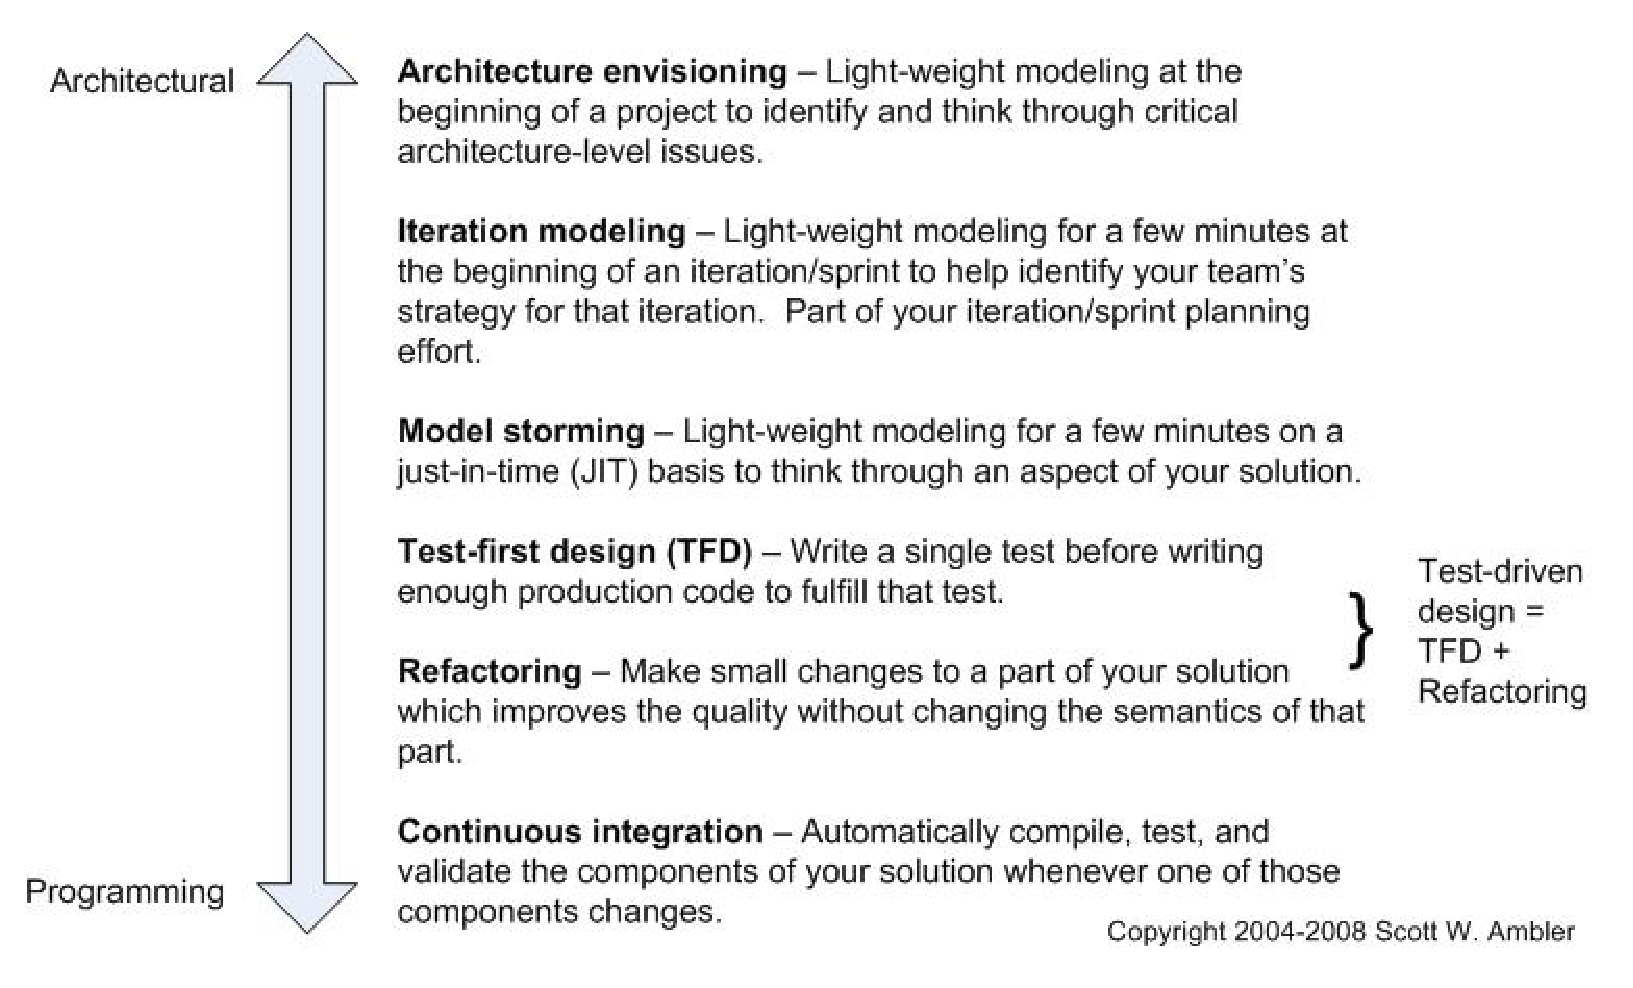
\includegraphics[width=0.8\textwidth]{agile_design_practices.eps}
\caption{Práticas do Design Ágil}
\label{fig:agile-design}
\end{figure}

%

O conjunto de práticas destacadas na Figura~\ref{fig:agile-design} podem ser utilizadas para a aplicação e exercicío dos princípios que são fundamentais para o desenvolvimento de um software que atenda a requisitos de qualidade do cliente, qualidade interna e proporcionem o sucesso em termos de custo e prazo. Quanto mais próximo do nível de abstração arquitetural, mais atenção é dada para os elementos e decisões genéricas do sistema. Por outro lado, quanto mais próximo do nível de programação, as práticas destacadas são aplicadas em elementos menores do software, sendo de suma importância para se conseguir os objetivos de nível arquitetural. Ainda a respeito de práticas como \emph{refactoring} e integração contínua vale ressaltar que estas são aplicadas constantemente pelos Engenheiros de Software, várias vezes por iteração até se atingir os objetivos funcionais e não-funcionais estabelecidos.

%

Durante as iterações e a aplicação das práticas da Figura~\ref{fig:agile-design}, outros elementos e técnicas de \emph{design} são importantes e devem ser considerados para se aplicar os princípios de \emph{design}. Paradigmas de programação, padrões de projetos, estilo de código e utilização de \emph{frameworks} são exemplos de elementos importantes para a concepção do \emph{design} de um sistema.

%

A definição do estilo ou padrão de programação é a escolha de um conjunto de regras e diretrizes para a escrita de um software, sendo fundamental para a propriedade coletiva do código. Um padrão de codificação implica que não há pessoalidade no código, facilitando a leitura e evolução do mesmo. Muitas vezes, a definição do padrão para um projeto se baseia em sugestões oferecidas pela comunidade de desenvolvimento de uma linguagem específica e em regras que a equipe de desenvolvimento consideram importantes para suportar a legibilidade, manutiblidade e impessoalidade do software. Estas regras devem estar documentadas e acessíveis para os desenvolvedores do projeto ou até mesmo estarem configuradas em ferramentas especializadas para suportar a aplicação de estilos de programação tal como o \emph{Checkstyle}\footnote{\url{http://checkstyle.sourceforge.net/}}. Kernighan \& Plauger (\citeyear{kernighan1978}) em seu livro \emph{The Elements of Programming Style} apresentam e avaliam elementos do estilo de programação de softwares reais, destacando lições aprendidas na análise dos códigos. A noção de padrões de código é extendida para o conceito de Código Limpo, explorado posteriormente nesta seção.

%

Tão importante quanto conhecer padrões e estilo de códigos é conhecer padrões de projetos para aplicação dos princípios de \emph{design}. Um padrão de projeto descreve uma solução geral reutilizável para um problema recorrente no desenvolvimento de sistemas de software que, geralmente, estão relacionados à algum paradigma específico. No conhecido livro \emph{Design Patterns: Elements of Reusable Object-Oriented Software}, Erich Gamma e seus colegas (\citeyear{gof1994}) definem que um padrão de projeto nomeia, abstrai e identifica os principais aspectos de uma estrutura comum de projeto útil para a criação de software reutilizável. A partir de um estudo empírico, Hegedüs e colaboradores (\citeyear{hegedus2012}) avaliaram os resultados obtidos a partir da aplição de alguns padrões de projetos em relação aos atributos de qualidade do ISO/IEC 9126 (\citeyear{iso9126}), onde foi observados impactos positivos sobre a manutenibilidade do software. Portanto, os padrões de projetos são ferramentas importantes para o desenvolvimento de softwares com aplicação dos bons princípios de \emph{design} e estabelecimento de uma arquitetura que seja reutilizável, extensível, manutenível, simples e modularizada. Os padrões de projeto devem ser considerados nas decisões em nível arquitetural e aplicados durante a implementação do software, por exemplo, a partir de refatorações como proposto em \cite{kerievsky2008}.

%

O apoio de \emph{frameworks} no desenvolvimento do sistema possui impacto direto na qualidade do software, seja esta desenvolvido para o projeto ou por terceiros. Os benefícios da utilização de \emph{frameworks} estão na melhoria da modularidade do sistema, reusabilidade, extensibilidade e inversão de controle provida para os desenvolvedores \cite{fayad1997}. Além disso, corroborando os benefícios da utilização de \emph{frameworks}, vale ressaltar que o desenvolvimento de \emph{frameworks} consiste na aplicação extrema de alguns padrões de projetos para provimento de alguns serviços e estabelecimento de controle de operações de uma aplicação, se tornando uma estrutura fundamental que vem sendo extremamente utilizado no desenvolvimento de sistemas \cite{fayad1997}.

%

% O paradigma Orientado a Objetos - OO se baseia na interação entre objetos conceituais que gerenciam seus próprios estados e operações. Dentre os conceitos mais importantes deste paradigma, destacam-se a classes, estrutura de herança, encapsulamento e o relacionamento entre objetos, conceitos estes que favorecem um \emph{design} modular, com maior flexibilidade ereusabilidade. Robert C. Martin introduziu cinco princípios básicos de \emph{design} OO conhecidos pelo acrônimo SOLID que tratam o gerenciamento de dependências entre os módulos do software:

% \begin{itemize}
% \item \textbf{\emph{Single Responsability principle}} - http://brizeno.wordpress.com/category/design-de-software/page/3/
% \item \textbf{\emph{Open/closed principle}} - 
% \item \textbf{\emph{Liskov substitution principle}} -
% \item \textbf{\emph{Interface segregation principle}} - http://brizeno.wordpress.com/2012/01/15/principios-de-design-de-software-interface-segregation-principle/
% \item \textbf{\emph{Dependency inversion principle}} - 
% \end{itemize}


\subsection{\emph{Code Smells} - Cheiros de Código}
\label{sec-bad-smells}

Um software pode ter sintomas (popularmente conhecido como \emph{Smells}) que podem indicar problemas relacionados ao uso de más práticas e a aplicação inadequada de princípios de \emph{design}. \emph{Code smells} não são a causa direta de falhas na aplicação, mas podem influenciar indiretamente para a inserção de erros responsáveis por futuras falhas \cite{fowler1999}. Em geral, eles são responsáveis pelas dificuldades de manutenção e evolução do sistema, realização de testes e propicia a inserção de \emph{bugs} \cite{mansoor2014}. Por isso, é muito importante saber como identificá-los para se aplicar os mecanismos necessários para sua remoção e, consequentemente, melhorar o \emph{design} do código existente. 

%

O tratamento de mals cheiros de códigos pode ser realizado preventivamente a partir do desenvolvimento da solução com pouca inserção de anomlias e características indesejáveis, a partir de aplicações de práticas de desenvolvimento e de princípios de \emph{design}. Por outro lado, também deve ser tratada constantemente a medida que o código é desenvolvido, através por exemplo da aplicação de \emph{refactorings} como proposto por \cite{fowler1999}. Para isso é necessária a identificação de suas ocorrências no código-fonte, que consiste na detecção de fragmentos de código que violam a estrutura ou propriedades semânticas desejadas, provocando acoplamento e complexidade, por exemplo \cite{mansoor2014}.

%

Martin Fowler em seu livro (\citeyear{fowler1999}), expõe que a identificação de mals cheiros de código (ou \emph{Bad Smells}) é o primeiro passo para realização de \emph{refactorings} controladas e em pequenos passos. Para tanto, ele explora quais são as principais ocorrências conhecidas de cheiros de códigos que devem ser tratados das quais iremos introduzir algumas:

\begin{itemize}
\item \textbf{Código Duplicado} - Mesma estrutura de código em mais de um lugar, indicando falta de reusabilidade.
\item \textbf{Método Longo} - Métodos longos com muitas linhas de código, indicando falta de modularidade, reusabilidade e baixa coesão, dificultando o entendimento do código.
\item \textbf{Classes Grande} - Classes que possuem muitas linhas de código, atributos e operações. Este mal cheiro indica falta de coesão na classe uma vez que as responsabilidades não são bem atribuídas.
\item \textbf{Lista Grande de Parâmetros} - Número grande de parâmetros passados para um método. Este mal cheiro dificulta o entendimento do código e do objetivo do método, podendo indicar também falta de coesão, uma vez que o objeto precisa de muitas informações externas para realizar suas operações internamente.
\item \textbf{Mudança Divergente} - Este mal cheiro acontece quando uma classe é constantemente modificada de diferentes formas por diferentes motivos. Mudanças Divergentes indicam que não há variações protegidas, demonstrando um alto acoplamento entre uma classe e a implementação de classes com quem ela se relaciona.
\item \textbf{Sirurgia de Espingarda} - Existe quando uma mudança realizada em uma classe afeta o funcionamento de outras estruturas. Este mau cheiro é bem semelhante à Mudanças Divergentes e ambos indicam os mesmos problemas.
\item \textbf{Dados Aglomerados} - Conjunto de atributos sempre são utilizados em conjunto seja em lista de parâmetros ou em operações em métodos. Este mal cheiro pode indicar uma falta de coesão relacionados a estes atributos, uma vez que seria mais interessante se estes atributos fossem compostos em um objeto mais apropriado para sua manipulação.
\item \textbf{Estruturas com \emph{Switch}} - Utilização da estrutura de seleção \emph{switch} em algumas linguagens. Este mal cheiro indica duplicação e falta de reutilização de código, uma vez que esta estrutura geralmente é utilizada repetidamente no código para realizar o mesmo controle de fluxo.
\item \textbf{Classes Preguiçosas} - Classes que não fazem o bastante para justificar sua existência. Este mal cheiro indica falta de coesão e pode indicar a existência de acoplamento desnecessário.
\item \textbf{Cadeias de Mensagens} - Existe quando um objeto solicita a outro objeto uma sequência de objetos para realizar alguma operação. Indica um forte acoplamento entre estas classes e aplicação inadequada do princípio de abstração.
\item \textbf{Heranças Recusadas} - Classes que recebem atributos e operações de suas classes mães, mas não gostariam de recebe-los. Esse mal cheiro indica a falta de encapsulamento e muito provavelmente a utilização inadequada de herança.
\end{itemize}

O entendimento e reconhecimento dos \emph{code smells} são muito importantes para que sua remoção seja feita o mais cedo possível no desenvolvimento. Entretanto, a identificação deles pode ser fragilizadas, pois dependem diretamente da interpretação e habilidade de identifação do desenvolvedor. Outro problema é não conhecer quais os mecanismos podem ser aplicados para a remoção destes mals cheiros de código. Neste sentido, o presente trabalho visa contribuir para o desenvolvimento de habilidades e ferramentas que possam ser utilizadas pelo Engenheiro de Software para encontrar as principais falhas de seus softwares e atuar de maneira a melhorar a qualidade interna dos mesmos.

\subsection{Código Limpo}
\label{sec-clean-code}

A definição de um bom código pode ser dada a partir de algumas características desejáveis para um código. No livro \emph{Clean Code} \cite{martin2008}, o autor aborda sobre um conjunto de características importantes que contribuem principalmente para um bom \emph{design} do código, sintetizando-os em um estilo de programação chamado Código Limpo. Este estilo de programação pode ser complementado pelas diretrizes propostas no livro \emph{Implementation Patterns} \cite{beck2007}, conforme estudado por Almeida \& Miranda (\citeyear{almeida2010}), pois ambos buscam a aplicação de três características:

%

\begin{itemize}
\item \textbf{Expressividade} - um código expressivo pode ser facilmente lido e deixa claro as intenções do autor através de operações e abstrações bem escolhidas. Esta expressividade permite a outros desenvolvedores compreender o código, modificar e utilizá-lo.
\item \textbf{Simplicidade} - simplicidade é também um dos principais princípios de \emph{design}, e diz respeito a redução de quantidade de informações que o leitor deve compreender para realizar alterações.
\item \textbf{Flexibilidade} - um código flexível permite que o software seja estendido sem que muitas alterações na estrutura deva ser feita.
\end{itemize}

%

Martin ressalva que para se conseguir um código expressivo, simples e flexível deve-se trabalhar em vários aspectos constantemente, desde o nome de métodos à estrutura da solução, pois a construção de um Código Limpo é iterativa e incremental. Esta ideia condiz com o modelo apresentado na Figura~\ref{fig:agile-design}. Portanto, um Código Limpo é resultado da constante evolução do código com cuidados sobre o seu \emph{design} com o exercício de práticas que aplicam os princípios de \emph{design}. 

%

Alguns aspectos importantes que devem ser sempre considerados para prover um código limpo são resumidas a seguir:

\begin{itemize}
\item \textbf{Nomes Significativos} - os desenvolvedores são responsáveis pela escolha de nomes de variáveis, classes e operações e, portanto, é de extrema importância que estes nomes revelem bem a intenção, diferenciando bem os elementos que compõe o software. Além disso, a escolha dos nomes são importantes para a abstração e compreensão dos diferentes módulos do software.
\item \textbf{Métodos Coesos} - métodos são fundamentais para o Código Limpo, pois encapsulam trechos de código, definem escopo de variáveis e são essenciais para a aplicação de princípios de \emph{design}. Neste sentido, há grande preocupação quanto ao tamanho dos métodos, reduzindo-se não só o número de linhas, mas principalmente a complexidade e número de responsabilidades.
\item \textbf{Argumentos Reduzidos} - é muito importante um número reduzido de argumentos dos métodos para facilitar sua compreensão, reduzir o esforço de testes e o acoplamento da classe com elementos externos.
\item \textbf{Classes Coesas} - as classes encapsulam dados e operações, sendo a principal estrutura que compõe o \emph{design} do software. É muito importante que as responsabilidades estejam bem definidas e distribuídas para cada classe de tal forma que haja menos dependências entre elas.
\end{itemize}

%

A composição de um Código Limpo é consequência da aplicação de princípios de \emph{design} e de boas práticas de programação. Um Código Limpo é, portanto, o estado desejável para que um software atenda os principais requisitos de qualidade interna. 

%ESCRVER ALGO MAIS?

%========================================================================================%

\section{Segurança de Software}
\label{sec-metrics-security}
%introdução

A segurança de software está relacionada com o contínuo processo de manter a confiabilidade, integridade e disponibilidade nas diversas camadas que o compõe, sendo considerado parte dos requisitos não-funcionais do sistema. Independentemente da criticidade do sistema, a segurança em software deve ser tratada com prioridade dentro do ciclo de vida de desenvolvimento do software. Aggarwal e colaboradores (\citeyear{aggarwal2002}) cita que o custo e esforço gastos na segurança do software são bem altos, podendo chegar a 70\% to esforço total de desenvolvimento e suporte do software.

%

Problemas de segurança são recorrentes em diversos tipos de sistemas podendo gerar perdas materiais e humanas em diferentes proporções. Vulnerabilidades em softwares são as maiores causas de infecção de computadores das coorporações e perda de dados importantes segundo a pesquisa Global Corporate IT Security Risks 2013 conduzido por B2B International em colaboração com Kaspersky Lab \cite{b2binternational2013}. Este estudo aponta que aproximadamente 85\% das empresas reportaram incidentes internos de segurança de TI. Mesmo com o grande esforço destinado a aspectos de segurança, tais problemas são difíceis de solucionar, pois a Engenharia de Segurança de Sistemas está em fase intermediária de desenvolvimento \cite{pascoa2002}. Gandhi e colaboradores (\citeyear{gandhi2013}) realçam as dificuldades de se detectar vulnerabilidades no estágio operacional do software, pois os problemas de segurança não são endereçados ou suficientemente conhecidos nas fases iniciais do desenvolvimento de software. 

%

Formalmente, uma vulnerabilidade pode ser definida como uma instância de uma falha na especificação, desenvolvimento ou configuração do software de tal forma que a sua execução pode violar políticas de segurança, implícita ou explícita \cite{krsul1998}. Vulnerabilidades podem ser maliciosamente exploradas para permitir acesso não autorizado, modificações de privilégios e negação de serviço. A exploração maliciosa de vulnerabilidades em grade parte são realizadas através de \emph{Exploits}, ferramentas ou scripts desenvolvidos para este propósito, que se baseiam extensivamente nas vulnerabilidades mais comuns tal como \emph{buffer-overflow}. 

%

Vulnerabilidades podem existir em diferentes níveis de um sistema, podendo, portanto, gerar problemas com diferentes proporções. Os níveis mais comuns suscetíveis a existência de vulnerabilidades são:

%

\begin{itemize}
\item \textbf{Hardware} - Vulnerabilidades relacionadas ao hardware de sistemas que estão expostos a humidade, poeira, calor, locais inseguros, dentre outros fatores físicos relacionados ao local onde se encontra a infra-estrutura de TI.
\item \textbf{Software} - Vulnerabilidades relacionadas às estruturas internas do software assim como aos dados que são acessados e processados. No geral, podem ser exercitados a partir de interações com o usuário não esperadas ou não validadas.
\item \textbf{Rede} - Vulnerabilidades relacionadas aos componentes da rede, tanto físicos (cabos, \emph{switches}) quanto em software (protocolos, dados). Este tipo de vulnerabilidade também está relacionada à falhas na comunicação como linhas de comunicação não protegidas, compartilhamento de informações com não interessados.
\item \textbf{Humana} - Vulnerabilidades relacionadas à processos que envolvem pessoas e níveis de acesso.
\item \textbf{Organizacional} - Vulnerabilidades relacionadas problemas em nível organizacional, principalmente relacionado à falta de políticas, auditorias e planos adequados.
\end{itemize}

%

No presente trabalho, estamos interessados essencialmente em vulnerabilidades de software. Mais especificamente, procuramos uma abordagem que facilite o tratamento destas vulnerabilidades dada sua importância e suas consequências. Neste sentido, faz-se necessário compreender quais são as ocorrências conhecidas de falhas de segurança em software e com quais vulnerabilidades estas falhas se relacionam.

%

Vulnerabilidades de software são, na maior parte das vezes, causadas pela falta ou imprópria validação das entradas realizadas pelo usuário. Essas condições indesejáveis são usadas por usuários maliciosos para injetar falhas e códigos no sistema que os permitam executar seus próprios códigos e aplicações  \cite{jimenez2009}. McGraw e colaboradores (\citeyear{mcgraw2004}) afirmam que 50\% dos problemas de segurança surgem no nível de design. Poucas ações específicas são tomadas por Engenheiros de Software para manter a segurança no desenvolvimento de novas funcionalidades ou até mesmo na realização de \emph{refactorings}. Em outras palavras, muitas vezes o Desenvolvedor de software pode estar inserindo vulnerabilidades no código que podem ser exploradas por usuários maliciosos ou, acidentalmente, por usuários comuns. Mesmo os Engenheiros de Software que realizam testes unitários automatizados tendem a não exercitar estas vulnerabilidades, pois no geral testam principalmente as condições de uso padrão do software, enquanto deveriam explorar melhor o comportamento do software à interações indesejadas \cite{vries2006}.

%

Algumas das vulnerabilidades mais comuns estão listada abaixo:

%

\begin{itemize}
\item \textbf{\emph{Buffer overflow}}: caso comum de violação de segurança da memória que ocorre normalmente quando dados são escritos em buffers de tamanhos fixos e ultrapassam os limites de memória definidos para eles. Como consequência, pode gerar mal funcionamento do sistema, já que o dado escrito pode corromper os dados de outros buffers ou até mesmo de outros processos, erros de acesso à memória, resultados incorretos e até mesmo interromper a execução do software. Esta vulnerabilidade também pode ser explorada para injetar códigos maliciosos, alterando a ordem de execução do programa para que o código malicioso tome controle do sistema. Algumas linguagens de programação oferecem mecanismos de proteção contra acesso ou sobrescrita da dados em qualquer parte da memória indesejada. Contudo, \emph{buffer ovewflows} ocorrem principalmente com programas escritos em C e C++ que não realizam a verificação automática se o dado a ser escrito em um \emph{array} cabe dentro dos limites de memória do mesmo.
%Podemos criar listagem de código 
\item \textbf{\emph{Dangling pointer}}: vulnerabilidade de violação de segurança da memória que ocorre quando um ponteiro não aponta para um objeto ou destino válido. Esta vulnerabilidade acontece ao se deletar um objeto ou desalocar a memória de um ponteiro sem modificar, entretanto, o valor deste ponteiro. Como resultado, o ponteiro ainda aponta para a mesma posição de memória que, por sua vez, já não está mais alocada para este processo. Como consequência, o sistema operacional pode realocar esta posição de memória para outro processo que, se acessado novamente pelo primeiro processo, irá conter dados incosistentes com o esperado. Em C e C++ esta vulnerabilidade existe também quando o ponteiro de um endereço de memória é declarado somente no escopo de um função e retornado por esta função. Muito provavelmente este endereço de memória será sobrescrito na pilha de alocação do processo pela chamada de funções posteriores. Além de incosistência de dados, esta vulnerabilidade pode ainda ser a causa de quebras de programas, como falhas de segmentação e pode ser explorada por ataques de injeção de código \cite{afek2007}. Algumas linguagens de programação como Java, Python e Ruby possuem um mecanismo de gerenciamento de destruição de objetos chamado \emph{Garbage Collector}\footnote{\url{http://www.informit.com/articles/article.aspx?p=30309&seqNum=6}}. 
%informações importantes sobre esta vulnerabilidade: https://www.usenix.org/legacy/events/sec10/tech/full_papers/Akritidis.pdf
%Seria interessante manter este footnote ou melhor referenciar como um Pattern do livro: http://www.informit.com/store/real-time-design-patterns-robust-scalable-architecture-9780201699562?w_ptgrevartcl=Real-Time+Design+Patterns%3a+Memory+Patterns_30309
%Listagem do código 
\item \textbf{\emph{Strings} formatadas não-controladas}: vulnerabilidade decorrida do tratamento inadequado das entradas do usuário sobre o software que, quando explorada, o dado submetido por uma \emph{string} de entrada é avaliado como um comando pela aplicação. Uma \emph{string} formatada pode conter dois tipos de dados: caracteres imprimíveis e diretivas de formatação de caracteres. Na linguagem C, funções de \emph{strings} formatadas tal como o \emph{printf} recebem um número variável de argumentos, dos quais uma \emph{string}  formatada é obrigatória. Para acessar o restante dos parâmetros que a chamada da função colocou na pilha, a função de \emph{string} formatada analiza a sequência de formatação e interpreta as diretrizes do formato a medida que realiza sua leitura \cite{lhee2002}.
\item \textbf{\emph{SQL Injection}}: vulnerabilidade presente em aplicações que aceitam dados de uma fonte não confiável, não os validando adequadamente e os usando posteriormente para construção de \emph{queries} dinâmicas de SQL para comunicação com o banco de dados da aplicação. Todos os tipos de sistemas que incorporam SQL estam sujeitos a esta vulnerabilidade, apesar de serem mais comuns em aplicações WEB. Como consequência da exploração desta vulnerabilidade tem-se a perda de confiabilidade e quebra de integridade dos dados de uma base de dados. Em alguns casos, a eploração de \emph{SQL Injection} pode permitir ao atacante levar vantagens através da persistência de informações e geração de conteúdos dinâmicos em páginas web \cite{uscert2012}.
\end{itemize}

%Lista: https://cwe.mitre.org/top25/
%http://nvd.nist.gov/cwe.cfm

\subsection{Classificações e taxonomias de vulnerabilidades}
\label{subsec-vulnerabilities-taxonomy}
%

O primeiro passo para que o desenvolvedor consiga cuidar de vulnerabilidades no código fonte é conhecer quais são os problemas mais comuns existentes em softwares e como os atancantes utilizam estas vulnerabilidadespara falhar o sistema. Existem muitos tipos de vulnerabilidades, e com o passar do tempo, novas vulnerabilidades são descobertas e novos \emph{exploits} são criados por atacantes. Em meio a essa diversidade, a classificação de vulnerabilidades representa um grande desafio, porém, já houve vários avanços na área com o objetivo de enumerar e catalogar estas vulnerabilidades.

%

O CVE (\emph{Common Vunerabilities and Exposures}) é um projeto criado pelo MITRE\footnote{\url{http://www.mitre.org/}} com o objetivo de enumerar as vulnerabilidades descoberdas pela comunidade para facilitar o compartilhamento de informações. Como é mostrado em \cite{cve2001martin}, antigamente cada organização nomeava de sua maneira uma vulnerabilidade, de forma que uma mesma vulnerabilidade era referenciada de maneira completamente distinta entra as organizações. 

%

A enumeração realizada pelo CVE é feita por uma junta de especialistas 	de segurança. Essa equipe nomeia, descreve e referencia cada nova ameaça. As novas ameaças são reportadas pela comunidade. Após estudo e aprovação, essa ameaça passa a incluir a lista da CVE, cujo o identificador é representado da seguinte forma : CVE-2014-0002. O valor 2014 significa que a CVE foi criada em 2014, e o numero 0002 se refere ao numero sequencial atribuído a essa CVE dentre todas que foram aprovadas nesse ano.

%

Surgiram propostas além do CVE para a classificação e agrupamento de vulnerabilidades, que são chamadas de taxonomias. O trabalho de Malerba (\citeyear{malerba2010}) descreve as as primeiras propostas taxonômicas, como os trabalhos de Landwher em 1992(\emph{A toxonomy of Computer Security Flaws}) e Aslam em 1997 (\emph{Use of  a taxonomy of Security Faults}). Porém, consideramos mais relevante abordar mais detalhadamente sobre as taxonomias mais recentes, que são utilizadas no projeto CWE, iniciativa semelhante a CVE que será abordada mais adiante. As principais taxonomias são:

%

\begin{itemize}
\item PLOVER (\emph{Preliminary List Of Vulnerability Examples for Researchers})
\item CLASP (\emph{Comprehensive, Lightweight Application Security Process})
\item \emph{Seven Pernicious Kingdom}
\end{itemize}

%

O PLOVER foi criado em 2005 pelo MITRE em parceria com o DHS (US. Departament of Homeland Secutity) e o NIST (National Institute of Technology). É um documento que lista mais de 1400 exemplos reais de vulnerabilidades identificados pelo CVE. Trata-se de um framework conceitual que descreve as vulnerabilidades em diversos níveis de detalhe. O PLOVER também fornece uma série de conceitos que podem ajudar na comunicação e discussões à respeitos de vulnerabilidades.

%

Foram definidas 28 categorias de mais alto nivel para a categorização de vulnerabilidades. Algumas dessas são:

\begin{itemize}
\item BUFF: inclui vulnerabilidades de Buffer Overflow, formatação de strings, etc;
\item CRIPTO: inclui vulnerabilidades relacionadas a criptografia;
\item SPECTS: inclui vulnerabilidades que ocorrem e tecnologias específicas, como a injeção de SQL e XSS
\end{itemize}

A lista completa das categorias e mais detalhes sobre o PLOVER podem ser encontrados em \cite{christey2006}.

%

O CLASP não é apenas uma taxonomia de categorização de vulnerabilidades, mas sim um processo que busca melhorar a segurança de softwares. No de diz respeito a classificação, o CLASP define 6 categorias alto nível que incluem 104 tipos de vulnerabilidades, que são:

\begin{itemize}
\item Erros de tipo e de Range
\item Problemas no ambiente 
\item Erros de sincronização e de temporização
\item Erros de protocolo
\item Erros de lógica
\item \emph{Malware}
\end{itemize}

%
Exemplificando, as vulnerabilidades do tipo \emph{Buffer Overflow} se encaixariam na categoria de erro de tipo e de range, pois nesse tipo de vulnerabilidade é permitido a escrita de uma informação além o limite do buffer. A vulnerabilidade do tipo  injeção de SQL também se encaixaria nessa categoria, pois esse tipo de vulnerabilidade ocorre quando não há validação no tipo de informação fornecida pelo usuário. Mais detalhes podem ser vistos no site do CWE\footnote{\url{http://cwe.mitre.org/about/sources.html}}.

%

A taxonomia Seven Pernicious Kingdoms é a que possibilita melhor entendimento ao desenvolvedor, e é até utilizada como base em uma das visões das CWEs denominada \emph{Development View}\footnote{\url{http://cwe.mitre.org/data/graphs/699.html}}. Utiliza os conceitos da biologia de Reino e Filo. Na taxonomia, o Reino é a classificação mais abrangente e o Filo é uma subdivisão do Reino. Essa taxonomia, embora o nome sugere sete, possui oito reinos sendo que sete reinos são dedicados a vulnerabilidades de código fonte e um reino referente a aspectos de configuração e ambiente. São eles:

\begin{itemize}
\item \textbf{Validação e representação de entrada}: inclui erros de buffer overflow, injeção de SQL, XSS, etc;
\item \textbf{Abuso de API}: Ocorre quando uma função que chama outra função assume certas condições que não estão garantidas pela rotina chamada.
\item \textbf{\emph{Features} de segurança}: está relacionado ao uso correto de peças chaves em segurança de código como criptografia, autenticação, gerenciamento de privilégios, etc;
\item \textbf{Tempo e estado}: está relacionado a erros de paralelismo, sincronização e uso de informação.
\item \textbf{Erros}: está relacionado erros oriundo da falta de tratamento de erros da aplicação.
\item \textbf{Qualidade de código}: são erros originados pela falta de qualidade no código fonte. Geralmente acontecem quando são utilizadas más praticas de programação que podem gerar colapso no sistema, como por exemplo não desalocar recursos não utilizados pode gerar \emph{Memory Leak};
\item \textbf{Encapsulamento}: são erros relacionados ao não estebelecimento de limite de acesso aos componentes do sistema
\item \textbf{Ambiente}: são erros que estão relacionados a fatores externos do software, que não estão no escopo deste trabalho.

\end{itemize}

A idéia desta taxonomia foi criar reinos bem amplos para que novos filos fossem inseridos em seu lugar correto, porém a taxonomia proposta está aberta para a inserção de novos reinos, caso necessário. Mais informações e detalhes a cerca dos filos que incluem cada reino pode ser encontrado em \cite{tsipenyuk2005}

%
Com este cenário apresentado acima, em que temos a CVE como projeto de enumerar as vulnerabilidades encontradas e as taxonomias elaboradas por diversos trabralhos com o objetivo de classificar e dar mais informações sobre a vulnerabilidade, ainda haviam a necessidade das empresas e organizações de utilizarem o uma terminologia padrão para listar e classificar vulnerabilidades de software, gerando uma linguagem unificada e uma base para ferramentas e serviços de medição dessas vulnerabilidades. Para essa necessidade foi elaborado o projeto CWE.

%
O CWE é uma lista formal de vulnerabilidades comuns de software (\emph{Common Weakness Enumeration}). Tem como objetivo estabelecer uma linguagem comum para descrever vulnerabilidades de software no design, arquitetura ou no código; servir de base para ferramentas de análise de cobertura de segurança de código, dessa forma é possivel saber quais vulnerabilidades as ferramentas conseguem capturar; e prover uma base de informações padrão a respeito de como identificar, mitigar e previnir uma certa vulnerabilidade. Dessa forma, diferente da enumeração fornecida pela CVE, O CWE também inclui detalhes sobre a vulnerabilidade e cria uma classificação baseadas nos trabalhos desenvolvidos sobre taxonomias apresentados neste trabalho e outros que não foram apresentados.
%

\subsection{Princípios de segurança}
\label{sec-security-principles}

Como visto no estudo sobre a classificação e taxonomias, existem muitas vulnerabilidades de software que são passíveis de exploração por atacantes. Neste sentido, é de suma importância para o desenvolvimento de softwares mais seguros que os Engenheiros de Software construam códigos com qualidade suficiente que os permitam identificar, corrigir e evitar a inserção de vulnerabilidades. Tendo-se o conhecimento de quais são as principais vulnerabilidades existentes, os Engenheiros devem tratar essas vulnerabilidades desde as primeiras fases de design e desenvolvimento código-fonte, seguindo até o fim do ciclo de vida do desenvolvimento do software. Assim como os desenvolvedores programam aplicando ao código princípios de design, devem evoluir o código aplicando princípios de design seguro tais quais os apresentados por outros trabalhos \cite{saltzer1975} \cite{bishop2003} \cite{mcgraw2002} \cite{a1lshammari2009}.

%

Dentre os princípios de segurança que os Engenheiros de Software podem aplicar no design de seus programas, introduziremos aqui os seguintes princípios:

\begin{itemize}
\item \textbf{\emph{Least privilege}}: este princípio sugere que o usuário deve ter somente os direitos necessários para completar suas tarefas \cite{bishop2003}. Em termos de design de classes, significa que o design mais seguro é aquele cujos métodos realizam o menor número de ações possíveis \cite{a1lshammari2009}.
\item \textbf{\emph{Reduce attack surface}}: este princípio tem como objetivo limitar o acesso a dados não permitidos. Pode-se aplicar este princípio reduzindo-se a quantidade de código executável, com \emph{design} prezando por menor números métodos de acesso (públicos) e menor número de parâmetros possíveis que possam afetar atributos privados para realização de uma tarefa. Pode-se também buscar eliminar serviços que são usados somente por poucos clientes.
\item \textbf{\emph{Defend in depth}}: este princípio sugere que os mecanismos de defesas devem ser aplicados na maior extensibilidade possível, mesmo que isso gere redundância. O princípio \emph{defend in depth} busca defender o sistema contra qualquer possível ataque através de implementação de métodos ou mecanismos diferentes de tratamento destes ataques. O \emph{design} em camadas facilita sua implementação, pois permite dividir os métodos de defesa de acordo com as responsabilidades de cada camada. Como ponto negativo, a implementação de vários mecanismos de defesa pode acrescentar complexidade ao software, aumentando riscos de inserção de outras vulnerabilidades e a dificuldade de encontrá-las.
\item \textbf{\emph{Fail securely}}: este princípio está relacionado ao controle das falhas que possam ocorrer na aplicação. As possíveis falhas existentes em um software devem ser exploradas e tratadas para que o software esteja preparado para responder a estas falhas adequadamente, sem gerar alarmes, quebrar a aplicação e principalmente abrir espaços para mais ataques maliciosos. Com a aplicação do princípio \emph{fail securely} tem-se a identificação e tratamento de erros, a inserção de mecanismos de respostas que facilitam a utilização correta do software e que permita que estes comportamentos sejam testados pelos desenvolvedores. Outra consequência positiva da aplicação deste princípio é que o princípio \emph{defend in depth} é apoiado uma vez que a identificação de possíveis erros reforça a modularização e separação dos métodos de tratamento dos mesmos.
\item \textbf{\emph{Economy of mechanism}}: princípio que se refere a manter o código que implementa mecanismos seguros menor e o mais simples possível. Este princípio é de suma importância para o tratamento de vulnerabilidades no desenvolvimento do software, pois a simplicidade é fundamental para que os Engenheiros de Software possam encontrar erros e corrigí-los. A medida que a complexidade aumenta, os módulos inseguros do software tendem a ficarem ocultos e mais difíceis de serem testados. A aplicação de técnicas de programação do XP tais como \emph{refactoring}, \emph{test-driven development} e programação em pares são fundamentais para alcançar os objetivos deste princípio. Este princípio está extremamente ligado ao princípio de design \emph{KISS - Keep It Simple, Stupid!}, pois ambos enfatizam que evitar a complexidade significa evitar problemas \cite{mcgraw2002}
\item \textbf{\emph{Mediate completely}}: princípio que defende que todos os acessos a quaisquer objetos devem ser verificados para garantir se há permissões para realizar tal ação. Se em algum momento for solicitado a leitura de um objeto, o sistema deve verificar se o sujeito tem permissão de leitura. Caso tenha, deve prover somente os recursos necessários para realização das tarefas que interessa a este sujeito. Esta operação deve se repetir todas as vezes que a requisição ao objeto for feita, não somente na primeira vez \cite{bishop2003}.
\item \textbf{\emph{Separation of duties}}: princípio relacionado a separação de interesses dentro dos métodos e mecanismos de segurança do software. A OWASP sugere a separação entre as entidades que aprovação a ação, entidades que realizam a ação e entidades que monitoram a ação \footnote{\url{https://www.owasp.org/index.php/Separation_of_duties}}. Este princípio está diretamente relacionado com os princípios de design orientado à objetos tais como coesão e separação de interesses. Por outro lado, também mantém forte relação com o princípio de design seguro \emph{Economy of mechanism}, pois proporciona código mais limpo e que podem ser mantidos separadamente.
\end{itemize}


Alguns módulos do software requerem mais atenção do que outros quanto riscos de vulnerabilidades. Neste sentido, principalmente em atividades de manutenção e evolução de um software existente, pode ser necessária a priorização do esforço para evolução da segurança do código-fonte voltados para módulos com maior risco. Pode-se, por exemplo, priorizar a redução da superfície de ataque em módulos mais expostos. Howard (\citeyear{howard2006}) propôs, dentre outras, as seguintes heurísticas para priorização da revisão de segurança de códigos:

%

\begin{itemize}
\item \textbf{Códigos antigos}: códigos mais antigos podem ter mais vulnerabilidades do que códigos produzidos recentementes. Isto acontece devido a evolução do entendimento da equipe de desenvolvimento quanto aos possíveis problemas de segurança. Além disso, Howard ainda enfatiza que qualquer código legado deve ser profundamente investigado.
\item \textbf{Códigos anonimamente acessíveis}: códigos que podem ser acessados por qualquer usuário, mesmo não autenticado, devem ser cuidadosamente revisados.
\item \textbf{Códigos que escutam em interfaces de rede globalmente acessíveis}: códigos que escutam as interfaces acessíveis de redes por padrão, principalmente de redes desconhecidas como a Internet, devem ser cuidadosamente revisadas e ter monitoramento de vulnerabilidades.
\item \textbf{Códigos escritos nas linguagens C, C++ e Assembly}: essas linguagens de programação possuem mecanismos de acesso direto à memória e devem ser periodicamente revisadas quanto a vulnerabilidades de \emph{buffer overflow} e de ponteiros inválidos ou inapropriadamente desalocados.
\item \textbf{Códigos com histórico de vulnerabilidades}: códigos que já apresentaram problemas de vulnerabilidade devem sempre ser foco de novas revisões, a não ser que possa ser demonstrado que as vulnerabilidades apresentadas já foram realmente removidas.
\item \textbf{Códigos que processam dados sensíveis}: códigos que manipulam dados sensíveis devem ser revisados para garantir que existam vulnerabilidades que permitam o acesso indevido aos mesmos por usuários não confiáveis.
\item \textbf{Códigos complexos}: códigos que estrutura complexa devem ser periódicamente revisados para investigar possíveis melhorias que diminuam a complexidade. Como já destacado anteriormente nesta monografia, a complexidade é uma das principais inimigas da segurança e pode ocultar vulnerabilidades perigosas.
\item \textbf{Códigos que mudam frequentemente}: códigos instáveis que são passíveis a mudanças frequentes devem ser revisados a cada grande mudança, pois mudanças podem trazer a inserção de novos \emph{bugs} e vulnerabilidades.
\end{itemize}


%

O estudo sobre conceituação de vulnerabilidades conhecidas, de princípios de \emph{design} seguro e da revisão bibliográfica nos permite afirmar que o Engenheiro de Software é o principal responsável por manter a segurança de seus projetos. Este profissional deve se preocupar com os problemas de segurança desde os primeiros passos da concepção do código-fonte e \emph{design} até o desenvolvimento dos últimos testes automatizados. Verifica-se uma forte relação entre princípios de design de software com os princípios de \emph{design} seguro, onde a aplicação de ambos podem prover softwares mais robustos, extensíveis e seguros. 

%

Como já mencionado, as decisões de design são fundamentais para a concepção de um software seguro. Khan \& Khan (\citeyear{khan2010}) enfatizam que a complexidade é o maior desafio para desenvolvedores de software ao projetarem um produto de qualidade que cubra ao máximo aspectos de segurança. Os mesmos autores ainda definem que a complexidade de software orientados a objetos está relacionada principalmente a quantidade de parâmetros de design de um objeto e as relações estabelecidas entre os objetos do projeto. Da mesma forma, a complexidade é um dos principais problemas que afetam a qualidade interna do software, dificultando principalmente a manutenção e evolução do software. Mesmo a complexidade sendo uma propriedade da essência do software e não acidental, conforme afirmado por Brook (FAZER CITAÇÃO), é de suma importância que os desenvolvedores cuidem da complexidade de seus códigos, pois estes esforços reduzem os impactos negativos diretos sobre a estrutura interna do software assim como na segurança do mesmo. Para tanto, faz-se necessário a aplicação dos princípios de bom \emph{design} e de princípios de \emph{design} seguro através, por exemplo, da prática de \emph{refactorings} e aplicação de padrões de projeto. A seguir são listadas algumas características observáveis no \emph{design} do software que podem indicar complexidade \cite{khan2010}:

%

\begin{itemize}
\item Grande número de métodos específicos da aplicação de um objeto afeta a reusabilidade.
\item Árvores de herança profundas.
\item A grande quantidade de números de filhos de uma classe.
\item Alto acoplamento entre objetos.
\item Grande número de métodos públicos de um objeto.
\item Baixa coesão de classes. 
\end{itemize}

%

O encapsulamento é uma das principais características de projetos orientados a objetos, sendo fundamental para estabelecer critérios de relação entre as classes de um projeto. Em termos de segurança, esta é outra característica fundamental que deve ser cuidadosamente pensada no \emph{design}de de códigos seguros, pois se relaciona diretamente com os princípios \emph{reduce attack surface} e \emph{mediate completely}.

%



%

O nível de encapsulamento também está extritamente relacionado com o princípio \emph{mediate completely}, uma vez que um baixo grau de encapsulamento provê diferentes formas de interações com o objeto que, segundo este princípio, devem ser verificadas sempre. Quando se tem diversos pontos de interação com um objeto as verificações necessárias para prover uma interação segura devem ser mais complexas para explorar os perigos inerentes a cada um desses tipos de interação. Portanto, restringir acessos à alguns métodos e atributos públicos podem beneficiar a aplicação do princípio de \emph{design} seguro \emph{mediate completely}.

%

Os cuidados com o nível de encapsulamento das estruturas do software tem outros impactos sobre o \emph{design} seguro. A maior parte das decisões de design afetam a complexidade do código-fonte, o que também é verdade para decisões relacionadas a encapsulamentos de classes. A redução dos métodos de acesso diminui as opções de interação com um objeto, tornando a API do objeto mais simples, sendo que o mesmo pode ser dito para a diminuição de parâmetros. Complementarmente, o encapsulamento auxilia na redução do acoplamento entre classes, promovendo maior independência entre os módulos do projeto, aumentando a extensibilidade, manutenibilidade e testabilidade do código. A redução do acoplamento entre classes apoia o \emph{design} seguro, principalmente na detecção e tratamento de vulnerabilidades através de testes e aplicações dos princípios de \emph{design} seguro cujos impactos são mais facilmente gerenciáveis.

%

%Introduzir métricas

Os cuidados com o bom design do código-fonte são fundamentais para o desenvolvimento de códigos seguros. Entretanto, ações específicas devem ser realizadas com objetivos de tratar especificamente das vulnerabilidades inerentes ao código produzido. Em um cenário ideal, essas ações deveriam ser realizadas por Engenheiros de Software ao longo do desenvolvimento, como inspeções de código-fonte para busca de vulnerabilidades. Felizmente, existem estudos e padrões que buscam compreender e definir a existência de vulnerabilidades no software e de que maneiras podemos tratá-las. Tais estudos permitem a criação de ferramentas que automatizam a identificação de possíveis vulnerabilidades no software através de métricas obtidas com a análise estática do código-fonte que podem e devem ser utilizadas por Engenheiros de Software para apoiar a produção de softwares seguros, independentemente da criticidade do sistema. 

%

%Lista: http://www.first.org/cvss/cvss-guide.pdf

%

%========================================================================================%

\section{Métricas em Engenharia de Software}
\label{sec-metrics-esw} 
Tanto a existência de um bom \emph{design} quanto a de testes automatizados que exercitem as funcionalidades são características desejáveis em projetos de software. Boa parte das técnicas modernas da Engenharia de Software (CITAR TÉCNICAS) são voltadas para desenvolvimento com design que proporcione simplicidade, manutenibilidade e testabilidade. Mesmo que a maior parte dessas técnicas tenham sido disseminadas a partir do advento dos Métodos Ágeis e do Software Livre, cujo foco central está em atividades relacionadas ao código-fonte, elas são aplicáveis independentemente da metodologia de desenvolvimento utilizada \cite{meirelles2013metrics}. A valorização por softwares que atendam estes parâmetros de qualidade deve-se ao fato de sempre que o Engenheiro de Software está escrevendo novas linhas de código, um tempo significativo é gasto por ele na leitura e entendimento do código existente, muitas vezes desenvolvidos por outros Engenheiros. Martin (\citeyear{martin2008}) destaca que o código-fonte deve ser escrito para ser entendido principalmente por pessoas, e não pela máquina.

%

Neste sentido, o monitoramento da qualidade de código-fonte é fundamental e pode apoiar a utilização de técnicas de desenvolvimento que visam a melhoria contínua do código. Além disso, as métricas de código-fonte são muito importantes para projetos de software, pois estas podem ser utilizadas tanto como ferramenta para gestão do projeto quanto como referência técnica para tomada de decisões sobre o código-fonte.

%

Uma métrica, no âmbito da Engenharia de Software, provê uma forma de medir quantitativamente atributos relacionados as entidades do software e do processo de desenvolvimento. Assim, métricas são importantes ferramentas para avaliação da qualidade do código-fonte produzido e acompanhamento do projeto. Meirelles (\citeyear{meirelles2013metrics}) destaca que, com métricas de software, propõe-se uma melhoria de processo de gestão com identificação, medição e controle dos parâmetros essenciais do software.

%

Métricas de monitoramento de código-fonte possuem natureza objetiva e foram inicialmente concebidas para medir o tamanho e a complexidade do software \cite{henry1984kafura}\cite{troy1981zweben}\cite{yau1985zweben}. Outras métricas surgiram para avaliar softwares que utilizam paradigmas específicos, não sendo aplicáveis a qualquer tipo de software. Por exemplo, métricas orientada a objetos são usadas para avaliar sistemas orientados a objetos \cite{systa2000}. Métricas OO são destinadas, portanto, para avaliar a coesão de classes, as hierarquias de classes existentes, nível de acoplamento entre classes, reuso de código, dentre outras características.

%

Algumas características importantes ajudam a classificar as métricas de código-fonte. Assim, podemos classificá-las como estáticas e dinâmicas. Como o próprio nome diz, métricas estáticas capturam propriedades estáticas dos componentes de software e não necessita que o software seja executado para que seus valores sejam coletados. Por outro lado, métricas dinâmicas refletem características chaves tais como dependência dinâmica entre os componentes em tempo de execução do software.

%

No contexto desta monografia estamos interessados principalmente na análise estática de códigos-fontes. Neste sentido, a análise estática é definida como o processo de avaliar um sistema ou seus componentes baseados em suas formas, estruturas, conteúdo ou documentação que podem gerar insumos para compreensão da qualidade de design do código assim como enderaçar suas principais vulnerabilidades, podendo ser realizada sobre módulos e até mesmo sobre códigos ainda não finalizados \cite{black2009}. Esta análise pode ser realizada manualmente, tal como é feita em inspeções de código e com \emph{pair programming} ou de maneira automatizada através de ferramentas desenvolvidas para tal fim (PRECISA CITAR FERRAMENTAS???). 

%

As métricas de software também podem ser classificadas quanto ao método de obtenção. Métricas primitivas podem ser diretamente coletadas refletindo um valor observável de um atributo, sendo raramente interpretadas independentemente. Por outro lado, métricas compostas são obtidas a partir da relação de uma ou mais métricas, derivada, por exemplo, a partir de uma expressão matemática.

%

Entretanto, as definições de métricas adequadas para o acompanhamento do projeto, dimensionamento do software e principalmente para a aferimento da qualidade do código-fonte são tarefas que aumentam a complexidade de adoção de métricas em projetos de software, assim como destacado por Rakić e Budimac (\citeyear{rakic2011budimac}). Isto se deve a diversos fatores: à grande quantidade de métrica existentes; pouca aderência de algumas métricas com a realidade; diversas formas de interpretação de dados; dificuldades de definir parâmetros para comparação; poucos recursos de visualização de dados; coleta de dados não automatizados ou difíceis. Fenton e Pfleeger (\citeyear{fenton1998}) definem características desejáveis de métricas que orientam a escolha das mesmas enquanto outros autores \cite{meirelles2013metrics}\cite{almeida2010} estudam formas de viabilizar a utilização de métricas pelos desenvolvedores em geral. O presente trabalho visa correlacionar métricas de desenvolvimento de software com objetivo de definir configurações para estabelecer cenários que representem o estado da qualidade do software. Desta forma, espera-se reduzir as dificuldades de utilização de métricas de código fonte, tanto para o acompanhamento gerencial quanto para a tomada de decisões de design por desenvolvedores baseada em evidências. Para tanto, nas próximas seções serão apresentados estudos realizados sobre métricas de monitoramento de código-fonte para sistemas orientados à objetos e métricas para avaliação de vulnerabilidades do software.

%

\subsection{Métricas Estáticas de Design de Software}

Nesta sub-seção iremos apresentar um conjunto de métricas de código-fonte que estão diretamente relacionadas ao \emph{design} de software. Neste conjunto de métricas estamos incluindo métricas que mensuram atributos do software tais como tamanho, complexidade assim como características específicas relacionadas à orientação à objetos. Portanto, métricas de \emph{design} de software devem ser compreendidas como um conjunto de métricas que medem atributos do código-fonte que permitam a avaliação de produtos de software.

%

A escolha de métricas para mensurar os atributos de \emph{design} se torna complexa, pois existem inúmeras propostas de métricas diferentes destinadas a medir os mesmo atributos, principalmente sobre tamanho e complexidade. Li \& Cheung \citeyear{li1987}, por exemplo, referencia e compara 31 métricas diferentes de complexidade. Entretanto, não está no escopo deste trabalho realizar uma comparação detalhada sobre métricas semelhantes. As métricas que iremos apresentar a seguir foram selecionadas devido a sua vasta utilização em estudos científicos referenciados neste trabalho e devido a sua existência em boa parte das ferramentas extratoras de métricas de código-fonte. Primeiramente serão apresentadas métricas relacionados a tamanho.

%

\begin{itemize}
\item \textbf{LOC (\emph{Lines of Codes} - Linhas de Código)}: LOC calcula o número de linhas executáveis, desconsiderando linhas em branco e comentários. Esta é a métrica de tamanho mais comum. Entretanto, deve ser cuidadosamente usada e composta, pois os parâmetros de comparação não devem ser os mesmos quando se varia a linguagem e estilo de programação.
\item \textbf{(\emph{Total Number of Modules or Classes} - Número Total de Módulos ou Classes)}: Esta métrica mensura o tamanho do software baseados na quantidade de módulos e classes, sendo menos sensível por linguagens de programação, nível de desenvolvedores e estilo de codificação \cite{meirelles2013metrics}.
\item \textbf{AMLOC (\emph{Average Method LOC} - Média de Número de Linhas de Código por Método)}: Esta métrica avalia a distribuição do código entre os métodos, sendo uma importante indicador de coesão, reutilização e outras características importantes. Entretanto, assim como a LOC, deve ser avaliada considerando-se a linguagem e estilo de programação.
\end{itemize}

%

As métricas de tamanho são muito importantes para a composição de novas métricas que permitam avaliar outras características do código-fonte. A seguir são apresentadas algumas métricas que avaliam atributos estruturais, sendo muito importantes para a compreensão do nível da qualidade do \emph{design}, principalmente manutenibilidade, flexibilidade e testabilidade.

%

\begin{itemize}
\item \textbf{NOA (\emph{Number of Attributes} - Número de Atributos)}: NOA calcula o número de atributos de uma classe, sendo bastante importante para avaliar a coesão de uma classe.
\item \textbf{(\emph{Total Number of Modules or Classes} - Número Total de Módulos ou Classes)}: Esta métrica mensura o tamanho do software baseados na quantidade de módulos e classes, sendo menos sensível por linguagens de programação, nível de desenvolvedores e estilo de codificação \cite{meirelles2013metrics}.
\item \textbf{NOM (\emph{Number of Methods} - Número de Métodos)}: Esta métrica se refere ao tamanho de uma classe medindo a quantidade de operações de uma classe. Sua interpretação pode ser complicada. Um número excessivo de métodos pode representar falta de coesão e de potencial de reusabilidade da classe. Por outro lado, pode representar uma classe bem estruturada com operações bem definidas. Entretanto, a avaliação isolada desta métrica não permite este tipo de afirmação.
\item \textbf{NPA (\emph{Number of Public Attributes} - Número de Atributos Públicos)}: NPA mede basicamente o encapsulamento de uma classe. Independente da linguagem, é desejado que este valor seja o mais baixo possível, pois é recomendado que a manipulação de atributos de uma classe sejam realizados por métodos de acesso e operacionais.
\item \textbf{NPM (\emph{Number of Public Methods} - Número de Métodos Públicos)}: Esta métrica é muito importante para a compreensão da abstração da classe, pois mede diretamente o tamanho da interface de acesso à mesma. NPM pode ser melhor utilizada para compreender o potencial de reusabilidade e coesão de uma classe do que a métrica NOM isoladamente.
\item \textbf{ANPM (\emph{Average Number of Parameters per Method} - Média de Parâmetros por Método)}: Essa métrica calcula a média de parâmetros dos métodos da classe, onde não se deseja um valor alto.
\item \textbf{MNPM (\emph{Maximum Number of Parameters per Method} - Número Máximo de Parâmetros por Método)}: Essa métrica corresponde à maior ocorrência de número de parâmetros dos métodos de uma classe.
\item \textbf{DIT (\emph{Depth of Inheritance Tree} - Profundidade da Árvore de Herança)}: Está métrica consiste no número de classes ancestrais da classe em análise, sem considerar heranças provindas de \emph{frameworks} ou bibliotecas. Para linguagens com herança múltipla, o valor desta métrica é o DIT da maior hierarquia.
\item \textbf{NOC (\emph{Number of Children} - Número de Filhos)}: NOC consiste no número de filhos direto de uma classe.
\item \textbf{ACCM (\emph{Average Cyclomatic Complexity per Method} - Média da Complexidade Ciclomática por Método)}: Esta métrica mede a complexidade média dos métodos de uma classe, baseando-se na complexidade dos fluxos de controle existente no método.
\end{itemize}

%

As últimas métricas que serão apresentadas nesta sub-seção buscam medir características discutidas anteriormente tais como coesão e acoplamento.

%

\begin{itemize}
\item \textbf{RFC (\emph{Response For a Class} - Resposta de uma Classe)}: Esta métrica mede a complexidade de uma classe contando o número de métodos que um objeto de uma classe pode invocar, tanto métodos internos quanto de outras classes.
\item \textbf{ACC (\emph{Afferent Connections per Class} - Conexões Aferentes por Classe)}: Esta métrica mede a conectividade de uma classe a partir da contagem de quantas classes do sistema acessam um atributo ou método da classe em análise. Caso o valor de ACC de uma classe seja alto, modificações em sua estrutura podem afetar mais classes.
\item \textbf{CBO (\emph{Coupling Between Objects} - Acoplamento Entre Objetos)}: Esta métrica calcula de quantas classes a classe em análise depende, sendo a recíproca da ACC.
\item \textbf{COF (\emph{Coupling Factor} - Fator de Acoplamento)}: Esta métrica é a razão entre o número acoplamento existente que não sejam provindos de herança e do número total de possíveis acoplamentos. O máximo de acoplamento possível acontece quando todas as classes estão e são acopladas com as outras classes do projeto.
\item \textbf{LCOM4 (\emph{Lack of Cohesion in Methods} - Ausência de Coesões em Métodos)}: Esta métrica cálcula o número de componentes conectados em uma classe. Um componente conectado consiste em um conjunto de métodos relacionados. Dois métodos são relacionados se ambos acessam as mesmas variáveis da classe ou um método invoca ao outro.
\end{itemize}


\subsection{Métricas Estáticas de Segurança}
\label{subsec-security-metrics}

Atualmente existem várias ferramentas de análise estática que detectam vulnerabilidades no código fonte. Essas ferramentas utilizam de divesas técnicas de detecção e buscam encontrar tipos específicos de vulnerabilidades. Como visto na Seção \ref{sec-metrics-security}, o projeto CWE busca definir  e classificar vulnerabilidades descobertas pela comunidade levando em consideração os detalhes de como essa vulnerabilidade ocorre no código para a geração de um erro. Considerando como referência o projeto CWE, vamos tomar como exemplo o erro de \emph{Buffer overflow}. Existem várias CWEs que especificam uma maneira diferente de se ter o erro de \emph{Buffer overflow}. Dessa forma, as ferramentas de análise estática buscam  encontrar vulnerabilidades específicas, considerando o padrão CWE ou não, para caracterizar a vulnerabilidade e quantificar o seu número de ocorrências. 

O uso de ferramentas de análise estática de código para a identificação de vulnerabilidades é uma alternativa muito interessante ao desenvolvedor, visto que é muito difícil para alguém que não tem muito conhecimento a respeito de vulnerabilidades de código fonte saber se está inserindo ou não uma vulnerabilidade no software. O trabalho de Aranha(\citeyear{aranha2012}) mostra claramente a importancia do uso de ferramentas de análise estática para a identificação de vulnerabilidades, visto que uma vulnerabilidade indentificada no software da urna eletronica utilizadas em votações no Brasil podia ter sido facilmente identificada e tratada se fossem utilizadas ferramentas de análise estática de código.

%

Então, em termos de métricas, ferramentas de análise estáticas podem fornecer as seguintes métricas relacionadas a vulnerabilidades:

\begin{itemize}
\item Número total de vulnerabilidades no projeto
\item Número de vulnerabilidades por arquivo
\item Número de vulnerabilidades por função
\item Quantidade de um vulnerabilidade especifica no projeto
\item Quantidade de um vulnerabilidade especifica por arquivo
\item Quantidade de um vulnerabilidade especifica por função
\end{itemize}

%
%metricas do analizo
Abaixo seguem algumas vulnerabilidades que podem ser encontradas e quantificadas	 por ferramentas de análise estática de código para linguagem C e C++, linguagens que oferecem uma grande flexibilidade ao programador, favorecendo a itrodução de vulnerabilidades.

\begin{itemize}
\item \textbf{\emph{UninitializedArgumentValue (uav)}}: Esta métrica conta as variáveis não inicializadas no código. As linguagens C e C++ não são inicializadas com valores \emph{default} quando são declaradas (recurso que é disponível em algumas linguagens) fazendo com que essas contenham lixo em seu conteúdo caso não sejam inicializadas. Dessa forma, a aplicação pode ter um comportamento inesperado quando utilizar essa variável não inicializada.

%

\item \textbf{\emph{Return of stack variable address (rsva)}}: Esta vulnerabilidade acontece quando uma função retorna um endereço para uma variável que está alocada na pilha (\emph{stack}). A pilha é o local onde variáveis temporárias são armazenadas, como por exemplo variáveis declaradas dentro de funções. Se uma função declara uma variável dentro de seu escopo e usa esta mesma para seu retorno, temos o retorno de uma variável alocada na pilha. Ao termino da execução da função, a área de memória utilizada por ela fica disponível. Dessa forma, a próxima função chamada pode utilizar esse espaço de memória, sobrescrevendo o conteúdo que anteriomente foi retornado pela função anterior. Logo, o ponteiro retornado pela primeira função pode ter o valor alterado, podendo gerar comportamento inesperado no sistema ou até a quebra da aplicação. Este tipo de vulnerabilidade é dificil de se identificar, sendo aconselhável o uso de ferramentas de análise estática de código.

%

\item \textbf{\emph{Potential insecure temporary file in call "mktemp" (pitfc)}}: Esta vulnerabilidade ocorre quando um arquivo temporário inseguro é criado e usado pela aplicação, tornando a aplicação e o sistema de dados vuneráveis a ataques.Um arquivo criado pela aplicação é considerado inseguro quando ele é criado por mecanismos (funções específicas de APIs) que não geram arquivos com nomes únicos ou com nomes de randomização fraca. A função "mktemp" é um exemplo de mecanismo de geração de arquivos temporários que gera um nome único para um arquivo com base em um prefixo definido no código fonte. Porém, essa randomização gerada pelo mktemp é fraca, de maneira que outra aplicação maliciosa pode usar o mktemp passando o mesmo prefixo e conseguir gerar um arquivo com o mesmo nome que pode conter código malicioso, ou mesmo utilizar deste arquivo para obter as informações que seriam salvas pela aplicação original.

%

\item \textbf{\emph{Potential buffer overflow in call to \'gets\' (fgbo)}}: Esta vulnerabilidade está relacionada ao uso da função "gets" da linguagem C que copia toda informação passada pela entrada do programa para um buffer sem checar se o tamanho da entrada é equivalente ao tamanho do buffer. Dessa forma, caso a entrada seja maior que o buffer, haverá a sobrescrita da memória adjacente. Isso pode resultar em comportamento errado do programa, incluindo erros de acesso à memória, resultados incorretos, parada total do sistema, ou uma brecha num sistema de segurança.

%

\item \textbf{\emph{Allocator sizeof operand mismatch (asom)}}:Esta vulnerabilidade consiste em passar o operador inadequado para o tamanho de uma alocação de memória. Por exemplo, a vulnerabilidade ocorre quando temos um ponteiro para int e no momento de alocarmos a memória passarmos no sizeof um tipo char. Esse tipo de situação pode gerar um buffer overflow no momento da atribuição da variável.

%

\item \textbf{\emph{Dereference of undefined pointer value (dupv)}}:Esta vulnerabilidade ocorre quando um ponteiro que não foi inicializado é acessado. Esta vulnerabilidade está relacionada a CWE 457 (Use Unitialized of variable) pois o ponteiro está indefindo pois não foi inicializado. Portanto, as consequencias podem ser desde a leitura de lixo de memória até mesmo a falha da aplicação.

%

\item \textbf{\emph{Divisions by zero (dbz)}}: Esta vulnerabilidade acontece quando existe uma divisão de um valor por zero. Quando temos essa situação, o programa para de funcionar. Essa vulnerabilidade geralmente acontece quando um valor inesperado é passado para divisor do cálculo ou ocorre algum erro que gere este valor. O melhor jeito de previnir é a realizar uma verificação que cheque se o divisor não é zero, e caso seja, deve-se implementar um tratamento, como por exemplo, o lançamento de excessoes.

%

\item \textbf{\emph{Memory leak (mlk)}}: O software não gerencia o uso de memória, provocando o consumo exessivo desta, podendo haver a falta de memória para a aplicação. Sem memória, a aplicação consegue funcionar corretamente, podendo gerar resultados inesperados como também a falha da aplicação.

%

\item \textbf{\emph{Out-of-bound array access (obaa)}}:Esta vulnerabilidade acontece quando a aplicação tenta acessar um indice de array que está fora de seu range. O acesso de uma posição fora do array pode causar falha na execução (por exemplo, na linguagem C, falha de segmentação) como também a execução de código, pois a região de memória acessada pode conter condigo a ser executado ou até outras informações, impactando na confidencialidade de dados.

%

\item \textbf{\emph{Double free (df)}}: Esta vulnerabilidade ocorre na linguagem C, quando o programa realiza a chamada free() duas vezes para o mesmo ponteiro. Chamar duas vezes o free() para o mesmo ponteiro pode corromper a estrutura de dados do programa que gerencia a memória. Esse erro ocorre normalmente em encadeamentos de estruturas condicionais má construidas.

\item \textbf{Assigned value is garbage or undefined (auv)}:Esta vunerabilidade ocorre quando não temos certeza que o valor atribuido existe. Esta vulnerabilidade ocorre quando uma variável recebe um valor cujo a origem vem de entrada do usuário no sistema. Caso não seja feito a verificação desse parâmetro de entrada, a variável poderá receber lixo ou um valor indefinido e sua posterior utilização pode causar desde quebra da aplicação como também resultados inesperados de comportamento de software.

\end{itemize}

 %SANS Institute, MITRE, e experts em segurança de software dos Estados Unidos e Europa elaboraram uma lista dos 25 erros de software mais perigosos. É uma lista que contem os erros mais comuns e perigosos que podem gerar sérias vulnerabilidades de software e que são muitas vezes fáceis de encontrar e de fácil exploit (REFERENCIA PARA SITE DA CWE). Estes erros são perigos pois podem permitir aos atacantes assumir o controle completo do software, roubar dados ou deixar a aplicação fora funcionamento. 
%

%Continuando com o exemplo da vulnerabilidade de Buffer Overflow, podemos citar duas CWEs que identificam essa vulnerabilidade de maneiras diferentes: CWE 242 e CWE 120. A CWE 120 é denominada \emph{Classic Buffer Overflow}, e esta vulnerabilidade ocorre quando quando um buffer de entrada é copiado para um buffer de saída sem que haja a verificação o tamanho da entrada é menor ou igual ao tamanho de saída, podendo gerar uma sobrescrita nas posições de memória além das posições utilizadas pelo buffer. Da mesma maneira, a CWE 242 também trata o risco de um buffer overflow com o uso da função "gets()" da linguagem C, que  copia os dados de input do usuário para um buffer, sendo que não há garantia de que o input será menor ou igual o limite do buffer destinado ao armazenamento da informação.

%

%A identificação desse códigos que representam vulnerabilidades específicas podem ser feitas com o auxílio de ferramentas de análise estática de código, justamente pelo fato de que é difícil para um programador saber se ele está inserindo uma vulnerabilidade no código ou não, pois é preciso ter o conhecimento da vulnerabilidade. A ferramenta de análise estática Analizo, por exemplo, fornece algumas métricas de vulnerabilidade. Estas são reportadas indicando a quantidade e o local de ocorrência.
%


\subsubsection{CVSS}

A medida que o código cresce e se torna mais complexo, faz-se necessário o uso de indicadores que auxiliem a visualização dos impactos de determinadas mudanças no código-fonte, inclusive em termos de possíveis vulnerabilidades que surgiram. Esses indicadores são obitidos a partir de interpretações de métricas que mensuram atributos relacionados ao código, seja de segurança ou não. 

O \emph{Common Vulnerability Scoring System - CVSS} é um \emph{framework} aberto desenvolvido pelo NIST (National Institute of Standard and Technology) em parceria com organizações industriais que endereça as questões relacionadas as métricas para quantificar a severidade e risco de vulnerabilidades \cite{cvss2007}. Com o CVSS é possível estabelecer um escore entre as vulnerabilidades de maneira que possa haver uma comparação entre a criticidade de cada vulnerabilidade para o contexto da organização. Distinguindo quais vulnerabilidades são mais graves, os gestores conseguem distribuir melhor o esforço para o tratamento dessas vulnerabilidades mais críticas. O CVSS é composto por três grupos de métricas: Básicas, Temporal e Ambiental. A seguir será dara uma breve descrição de cada métrica em cada um desses grupos. Mais informações sobre cada uma delas podem ser vistas no apendice.

%

O grupo de métricas Básicas capturam características intrínsecas e fundamentais de uma vulnerabilidade que são constantes no tempo e no ambiente de uso. As métricas que compõe esse grupo são:

\begin{itemize}
\item \textbf{Access Vector - AV}: esta métrica representa como a vulnerabilidade é explorada, localmente ou remotamente. Quanto mais remoto puder ser um ataque à informações de ativos, maior a pontuação da vulnerabilidade. Essa métrica pode assumir três valores: Local  (é necessário um acesso físico ou conta local), Rede Adjacente (é preciso ter acesso a uma rede local) e Rede (exploração remota).

\item \textbf{Access Complexity - AC}: algumas vulnerabilidades requerem alguns passos mais complexos para serem exploradas. Portanto, esta métrica mede a complexidade do ataque necessário para explorar a vulnerabilidade uma vez que o atacante tenha ganhado o controle sobre um sistema alvo. Essa métrica pode ter os seguintes valores: Alto, Médio e Baixo. Por exemplo, complexidade de acesso alta  indica que o atacante precisa de condições especiais, tal como privilégio de acesso; já complexidade baixa não requer nenhum privilégio de acesso para a exploração da vulnerabilidade
	
\item \textbf{Authentication - Au}: esta métrica mede a quantidade de vezes que um atacante deve ser autenticado para explorar um vulnerabilidade. Quanto menos autenticações, maior será o valor desta métrica. Vale destacar que o objetivo desta métrica não é medir a complexidade e segurança do mecanismo de autenticação. Os indicadores desta métrica são simples e bem definidos: Multíplo , indicando duas ou mais autenticações necessárias; Único, indicando que apenas uma auntenticação é realizada; e Nenhum , indicando que nenhum auntenticação é realizada.
\item \textbf{Confidentiality Impact - C}: esta métrica mede o impacto na confidencialidade do sistema quando uma vulnerabilidade é explorada. A confidencialidade refere-se a limitar o acesso a informações e sua divulgação somente para usuários autorizados. Os valores para essa métrica podem ser: Nenhum, indicando nenhum impacto na confidencialidade; Parcial, existe vazamento parcial da informação, porém o atacante não tem o controle sobre a informação; e Completa, indicando que o atacante possui total controle sobre as informações de todo o sistema.


\item \textbf{Integrity Impact - I}: esta métrica mede o impacto da integridade do dados após um \emph{exploit} realizado com sucesso. Intregridade se diz respeito a confiabilidade e veracidade da informação. Os valores para esta métrica podem ser: Nenhum, indicando que não há nenhum impacto; Parcial, indicando que o atacante não tem o controle de qual arquivo ele vai atacar; Completa, indicando que o atacante é capaz de modificar qualquer arquivo.
	

\item \textbf{Availability Impact - A}: essa métrica mede o impacto da disponibilidade do sistema após o ataque. Ataques que consomem a largura de banda da rede, o uso do processador ou espaço do disco possuem impacto direto com a disponibilidade do sistema. Os valores para esta métrica podem ser : Nenhum, indicando que não há impacto sobre a disponibilidade; Parcial, indicando que houve redução na performance ou interrupções no sistema; e Completa, indicando que o atancante conseguiu deixar os recursos da aplicação completamente indisponíveis.


%
As métricas do grupo Temporal podem ser desconsideradas do cálculo, sendo opcionais. Este grupo de métricas representam características de uma vulnerabilidade que podem mudar ao longo do tempo mas não mudam entre ambientes de usuário.



%

As métricas do grupo Ambiental também são opcionais ao calculo, podendo ser desconsideradas. Este grupo de métricas representam características de uma vulnerabilidade relevantes a um particular ambiente de usuário. Ou seja, são características que estão relacionadas unicamente ao ambiente em que a vulnerabilidade é analisada.
%  

%


COLOCAR EM APENDICE

vetor de acesso

\begin{table}[H]
	\begin{center}
	    \begin{tabular}{ | l | p{10cm} |}
	    \hline
	    Valor da Métrica & Descrição \\ \hline
	    Local (L) & Uma vulnerabilidade que só pode ser explorada com acesso local requer que o atacante tenha acesso físico ao sistema vulnerável ou a uma conta local (shell) \\ \hline
	    Rede Adjacente (A) & Uma vulnerabilidade explorável através de um acesso a rede adjacente exige que o atacante tenha acesso a partir de \emph{broadcast} ou colisão de domínios do software sob ataque \\ \hline
	    Rede (N) & Uma vulnerabilidade explorável através de acesso a rede significa que o software vulnerável está vinculado a rede e não requer que o atacante tenha acesso local, podendo realizar uma "eploração remota" \\ \hline
	    \end{tabular}
	    \caption{Avaliação de Indicadores da Métrica AV}
	    \label{tab:av_scoring}
	\end{center}
	\end{table}

Complexidade de acesso
	\begin{table}[H]
	\begin{center}
	    \begin{tabular}{ | l | p{10cm} |}
	    \hline
	    Valor da Métrica & Descrição \\ \hline
	    Alto (H) & Existem condições especiais de acesso tais como: ter o privilégio de acesso e o atacante deve explorar condições diferentes de uso do software. \\ \hline
	    Médio (M) & As condições de acessos são de alguma forma especiais tais como: a superfície vulnerável ao ataque só é acessível para um grupo de usuários e algumas informações devem estar disponíveis para possibilitar o ataque. \\ \hline
	    Baixo (L) & Não existem condições especiais de acesso permitindo ataques manuais por atacantes com poucas habilidades.\\ \hline
	    \end{tabular}
	    \caption{Avaliação de Indicadores da Métrica AC}
	    \label{tab:ac_scoring}
	\end{center}
	\end{table}

	Confidentiality Impact - C

	\begin{table}[H]
	\begin{center}
	    \begin{tabular}{ | l | p{10cm} |}
	    \hline
	    Valor da Métrica & Descrição \\ \hline
	    Nenhum (N) & Não há nenhum impacto sobre a confidencialidade do sistema. \\ \hline
	    Parcial (P) & Existe a divulgação considerável inapropriada de informações, mas o atacante não tem controle sobre a informação obtida.  \\ \hline
	    Completa (C) & Existe a divulgação total inapropriada de informações, onde o atacante pode obter informações de todo o sistema\\ \hline
	    \end{tabular}
	    \caption{Avaliação de Indicadores da Métrica C}
	    \label{tab:c_scoring}
	\end{center}
	\end{table}

	Integrity Impact - I
	\begin{table}[H]
	\begin{center}
	    \begin{tabular}{ | l | p{10cm} |}
	    \hline
	    Valor da Métrica & Descrição \\ \hline
	    Nenhum (N) & Não há nenhum impacto sobre a integridade do sistema. \\ \hline
	    Parcial (P) & Modificações de alguns arquivos são possiveis, porém o atacante não tem controle sobre o que pode ser modificado ou alcance do que pode ser modificado pelo atacante é limitado. Por exemplo, um sistema pode conter vários arquivos e o atancante não tem o controle de qual arquivo ele irá afetar.  \\ \hline
	    Completa (C) & O atacante é capaz de modificar qualquer arquivo do sistema\\ \hline
	    \end{tabular}
	    \caption{Avaliação de Indicadores da Métrica I}
	    \label{tab:i_scoring}
	\end{center}
	\end{table}


Disponibilidade do sistema
		\begin{table}[H]
	\begin{center}
	    \begin{tabular}{ | l | p{10cm} |}
	    \hline
	    Valor da Métrica & Descrição \\ \hline
	    Nenhum (N) & Não há nenhum impacto sobre a disponibilidade do sistema. \\ \hline
	    Parcial (P) & Existe redução na performance ou interrupções na disponibilidade do recurso. Por exemplo, um ataque que afetam a largura da banda reduz o número de conexões de usuários.\\ \hline
	    Completa (C) & O atacante é capaz de deixar o recurso completamente indisponível.\\ \hline
	    \end{tabular}
	    \caption{Avaliação de Indicadores da Métrica A}
	    \label{tab:a_scoring}
	\end{center}
	\end{table}
\end{itemize}